\newpage
\section{Training Neural Networks}

\subsection{Activation Functions}

\begin{figure}[!htb]
    \centering
    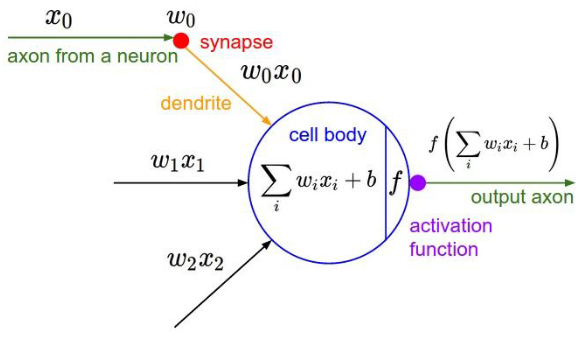
\includegraphics[width=0.42\textwidth]{pic/Lec6/a neuron}
    \caption{a neuron}
\end{figure}


\subsubsection{Sigmoid}
\begin{figure}[!htb]
    \centering
    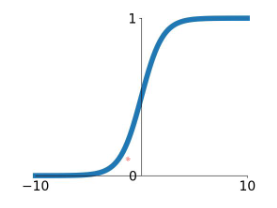
\includegraphics[width=0.309\textwidth]{pic/Lec6/Sigmoid.png}
    \caption{Sigmoid}
\end{figure}

\begin{align*}
    \sigma(x)=\frac{1}{1+e^{-x}}
\end{align*}

将数值压缩到 $[0,1]$. 历史上很受欢迎,因为它们被很好地解释为神经元的饱和``放电率''. 

\textbf{Problems}:
\begin{enumerate}
    \item 饱和神经元会杀死梯度. 在 $[-10,10]$ 以外的区域, $\sigma(x)$ 的梯度几乎是 $0$. 
    \item 其不以 $0$ 为平均 (没有负值), 这导致 参数 $\mathbf{w}$ 的梯度要么恒正要么恒负 (取决于初始的 $\mathbf{w}$ 的符号), 这会限制梯度更新的方向, 让学习更为低效. 所以希望 $x$ 以 $0$ 为平均. 
    \item $\exp$ 计算昂贵 
\end{enumerate}

\subsubsection{tanh}

\begin{figure}[!htb]
    \centering
    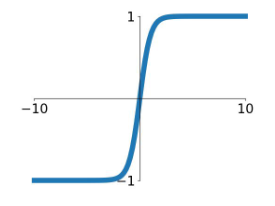
\includegraphics[width=0.309\textwidth]{pic/Lec6/tanh.png}
    \caption{$\tanh(x)$}
\end{figure}

压缩数值到 $[-1,1]$, 以 $0$ 为中心. 

Probelm: 饱和神经元仍会杀死梯度. 

\subsubsection{ReLU}
\begin{figure}[!htb]
    \centering
    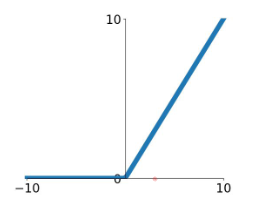
\includegraphics[width=0.309\textwidth]{pic/Lec6/ReLU.png}
    \caption{ReLU(Rectified Linear Unit)}
\end{figure}
\begin{align*}
    \text{ReLU}(x)=\max(0,x)
\end{align*}

在 $>0$ 时不会饱和, 计算高效, 收敛迅速(实验的结果), 在生物学上更合理. 

\textbf{Probelms}:
\begin{enumerate}
    \item 输出的平均值非 $0$.
    \item 负数无梯度. 可以给所有ReLU初始化一个极小的正偏置, 让其至少在更新?
\end{enumerate}


\subsubsection{Leaky ReLU}
\begin{figure}[!htb]
    \centering
    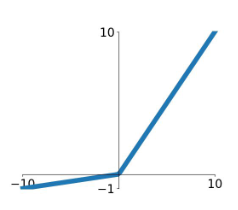
\includegraphics[width=0.309\textwidth]{pic/Lec6/Leaky ReLU}
    \caption{Leaky ReLU}
\end{figure}
\begin{align*}
    \text{Leaky ReLU}(x)=\max(0.01x, x)
\end{align*}

不会饱和, 计算高效, 收敛迅速(实验的结果), 且神经元不会死亡. 

Parametric Rectifier(PReLU)
\begin{align*}
    \text{PReLU}(x)=\max(\alpha x, x)
\end{align*}
对$\alpha$进行反向传播. 

\subsubsection{ELU}
\begin{figure}[!htb]
    \centering
    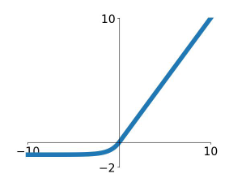
\includegraphics[width=0.309\textwidth]{pic/Lec6/ELU.png}
    \caption{ELU}
\end{figure}

\begin{align*}
    \text{ELU}(x)=\left\{ \begin{array}{ll}
        x & \text{if }x>0\\
        \alpha(e^x-1)&\text{if }x\le 0
    \end{array} \right.
\end{align*}

有 ReLU 的所有优点, 数据平均值更接近0, 相比 Leaky ReLU, 负饱和状态为噪声增加了些鲁棒性. 

Probelm: 计算需要 $\exp$. 

\subsubsection{Maxout}
\begin{align*}
    \max(w_1^Tx+b_1, w_2^Tx+b_2)
\end{align*}

没有点积的基本形式, 全局非线性. 囊括了 ReLU 与 Leaky ReLU. 局部线性, 不会饱和, 不会死亡. 

Problem: 参数翻倍. 

\subsection{Data Preprocessing}
\begin{figure}[!htb]
    \centering
    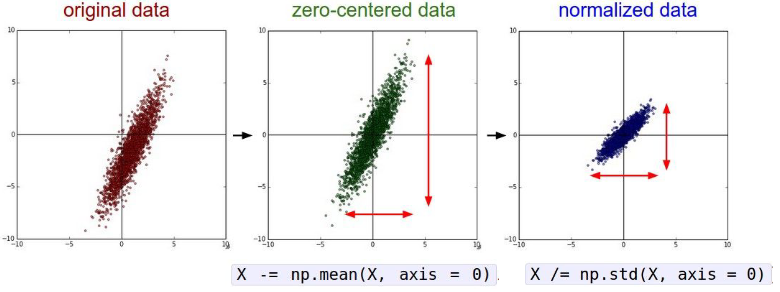
\includegraphics[width=0.42\textwidth]{pic/Lec6/Preprocess the data}
    \caption{Preprocess the data}
\end{figure}
值向0平均与归一化. 

\subsection{Weight Initialization}
尝试: 
\begin{enumerate}
    \item 若权重全初始化为0, 则大多数神经元会被同化(输入输出相同, 获得的梯度相同)
    \item 若权重被初始化为一个随机小值(平均值为0, 标准差为0.01的Gaussian随机), 对小网络还行, 对深度的网络不行.  因为输出会渐渐变小(因为小的参数), 导致网络会向0坍缩. 且因为参数小, 梯度也很小, 传播下来也坍缩为0了. 
    \item 若权重被初始化为一个随机值(平均值为0, 标准差为1的Gaussian随机), 几乎所有神经元都完全饱和, 梯度会消失. 
    \item 目的是使每一层的激活值的方差保持相同, 从而防止梯度爆炸或消失(数学推导假定线性激活). 
    \item 多个$/2$对ReLU进行调整. 
\end{enumerate}

正确的初始化还是很重要的. 

\subsection{Batch Normalization}
为了让每一层都是标准的gaussian, 使用
\begin{align*}
    \hat{x}^{(k)}=\frac{x^{(k)}-E\left[ x^{(k)} \right]}{\sqrt{\text{Var}\left[ x^{(k)} \right]}}
\end{align*}
此函数基本可微. 

在前向传播时:
\begin{enumerate}
    \item 计算每层计算的均值和方差
    \item Normalize (归一化)
\end{enumerate}

然后甚至可以再学两 squash 的参数:
\begin{align*}
    y^{(k)}=\gamma^{(k)}\hat{x}^{(k)}+\beta^{(k)}
\end{align*}
注: 这两个参数$\gamma^{(k)}, \beta^{(k)}$是有可能将 $\hat{x}^{(k)}$ 的归一化抵消的, 以此来学习调整归一化程度.

常插入在 全链接或卷积层之后, 在非线性层之前. 

改善网络梯度. 允许更高的学习率. 减少了对初始化的强依赖. 甚至是一种程度的正则化, 可以一定程度上替代 dropout?

再注: 测试时, 平均与方差是通过训练集估计的, 不是依赖于测试集. 


\subsection{Babysitting the Learning Process}
确认 loss 是合理的, 在特定的初始化下loss可以估计, 确认未训练的网络loss符合估计. 比如对于使用 Softmax loss 的 10 个类别的分类器, 初始的 loss 应该为 $-\ln \left( \frac{e^{0.1}}{10*e^{0.1}} \right)= -\ln 0.1 \approx 2.3$. 当再加入正则化时, loss也理应提升. 

\subsubsection{Try to train}
\begin{enumerate}
    \item 确保可以过拟合极小的数据. 
    \item 从小的正则化与学习率开始
    \subitem 学习率过小, loss不下降 (但准确率可能上升, 因为还是有在学的)
    \subitem 学习率过大, loss会爆炸
\end{enumerate}

\subsection{Hyperparameter Optimization}
\subsubsection{Cross-validation strategy}
在训练集上训练, 然后在测试集上测试. 在测试集上:
\begin{enumerate}
    \item 仅训练几个 epochs 来粗略观察参数是否有效
    \item 更长的训练, 更细的调整. 
\end{enumerate}
当调整后的 loss 超过原loss3倍以上, 可以不用再试了. 

可以调整:
\begin{itemize}
    \item 参数分布 (linear or log )
    \item 参数范围
    \item 参数的采样 (网格或随机)
\end{itemize}

\begin{figure}[!htb]
    \centering
    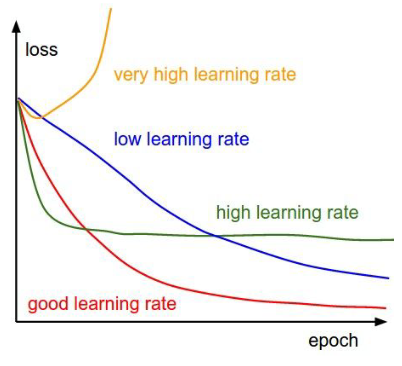
\includegraphics[width=0.309\textwidth]{pic/Lec6/learning rate.png}
    \caption{learning rate}
\end{figure}

loss 不变后突然下降: 可能是因为初始化不好. 